\chapter{Kolmogorov--Smirnov, Lilliefors and QQ Plots}
\label{ch:ks}

\begin{chaptergoals}
\begin{itemize}[nosep]
\item The empirical CDF, which estimates a whole distribution at once. At each point it is a sample proportion, so the Law of Large Numbers and the Central Limit Theorem apply point by point; the Glivenko--Cantelli theorem makes the first hold at all points at once, and Donsker's theorem does the same for the second.
\item The Kolmogorov--Smirnov test of a stated continuous distribution: the largest vertical gap between the empirical CDF and the candidate. Its null distribution is the same for every continuous candidate, so one table, or one simulation, serves them all.
\item Other measures of the gap, Cram\'er--von Mises and Anderson--Darling, and what binning the data for a chi-squared test gives up.
\item Testing a family: estimating its parameters changes the null distribution, and the Kolmogorov--Smirnov table then gives a test that almost never rejects. The Lilliefors test for normality is the repair.
\item QQ plots: the same comparison drawn as quantiles against quantiles, and how to read heavy tails, light tails and skew from one. Newcomb's measurements of the speed of light and the eruptions of Old Faithful.
\end{itemize}
\Cref{ch:gof} tested distributions on finitely many categories by counting. This chapter tests continuous distributions without grouping the data at all.
\end{chaptergoals}

\section{The empirical CDF}
\label{sec:ks-ecdf}

A continuous distribution has no natural categories.
\Cref{ch:gof} could still test one by cutting the line into cells and counting, but the answer depends on where the cuts go, and each observation is reduced to the name of its cell.
The object that describes a distribution on the line without any cutting is its CDF, $F(t) = \Pr(X \leq t)$, and it has an obvious estimate: the proportion of the sample at or below $t$.

\begin{definition}[The empirical CDF]
\label{def:ecdf}
For a sample $\Xton$, the \textbf{empirical CDF} is the random function
\[
F_n(t) = \frac1n\sum_{i=1}^n \ind(X_i \leq t) = \frac{\#\{i : X_i \leq t\}}{n}, \qquad t \in \real.
\]
With the observations sorted, $X_{(1)} \leq X_{(2)} \leq \cdots \leq X_{(n)}$ (the \textbf{order statistics}), $F_n$ is a staircase that is $0$ below $X_{(1)}$, climbs $1/n$ at each observation, and is $1$ from $X_{(n)}$ on.
\end{definition}

\begin{inwords}
\textbf{In words.} At each $t$, count the observations at or below $t$ and divide by $n$ \toolkit{sec:math-indicator}. The result is the CDF of the distribution that puts probability $1/n$ on each data point.
\par\smallskip
\textbf{For the kiss data.} With $R_i = 1$ for a right turn, $F_n(t)$ is $0$ for $t < 0$, $44/124 = 0.355$ for $0 \leq t < 1$, and $1$ from $t = 1$ on. Its step at $1$ has height $\hat{p} = 0.645$: for two-valued data the empirical CDF carries exactly the information in $\hat{p}$.
\end{inwords}

The left of \cref{fig:ecdfgc} shows two empirical CDFs of simulated waits from the exponential distribution with mean $6.23$ minutes, the model of the subway data, against the true CDF.
With $10$ observations the staircase is coarse and strays as far as $0.25$ from the curve; with $100$ it stays within about $0.08$.

\recall{The Law of Large Numbers (\cref{thm:wlln}): for i.i.d.\ random variables with mean $\mu$ and finite variance, $\bar{X}_n \convp \mu$. The Central Limit Theorem (\cref{thm:clt}): if the variance $\sigma^2$ is also positive, $\sqrt{n}(\bar{X}_n - \mu) \convd \Gauss(0, \sigma^2)$. Slutsky's theorem (\cref{thm:slutsky}): if $X_n \convd X$ and $Y_n \convp y$, a constant, then $X_nY_n \convd yX$; it lets an estimated standard error stand in for the true one.}

\begin{proposition}[The empirical CDF at fixed points]
\label{prop:ecdf-pointwise}
Let $\Xton$ be i.i.d.\ with CDF $F$. For each $t$, $nF_n(t) \sim \Bin(n, F(t))$, so $\E[F_n(t)] = F(t)$ and $\var(F_n(t)) = F(t)(1 - F(t))/n$; for $s \leq t$, $\cov(F_n(s), F_n(t)) = F(s)(1 - F(t))/n$. As $n \to \infty$, $F_n(t) \convp F(t)$, and if $0 < F(t) < 1$, $\sqrt{n}(F_n(t) - F(t)) \convd \Gauss\big(0, F(t)(1 - F(t))\big)$.
\end{proposition}

\optionalproof{$F_n(t)$ is the average of the i.i.d.\ indicators $\ind(X_i \leq t)$, each Bernoulli with mean $F(t)$; the Law of Large Numbers and the CLT do the rest.}
\begin{proof}
The indicators $\ind(X_i \leq t)$ are independent and each is $\Bern(F(t))$, so their sum $nF_n(t)$ is $\Bin(n, F(t))$, with mean $nF(t)$ and variance $nF(t)(1 - F(t))$.
For $s \leq t$, $\ind(X \leq s)\ind(X \leq t) = \ind(X \leq s)$, so the two indicators of one observation have covariance $F(s) - F(s)F(t) = F(s)(1 - F(t))$; indicators of different observations are independent, and dividing the sum of the $n$ covariances by $n^2$ gives the formula.
The two limits are the Law of Large Numbers and the CLT for the average of the indicators, whose variance $F(t)(1 - F(t))$ is finite, and positive when $0 < F(t) < 1$.
\end{proof}

So at any one point the empirical CDF is an ordinary proportion, and \cref{ch:confidence-intervals} already gives an interval for it.
For the waiting times between eruptions of Old Faithful (\cref{ch:likelihood}), $83$ of the $272$ waits were $60$ minutes or less, so $F_{272}(60) = 0.305$, and the plug-in $95\%$ interval for $F(60)$ is $0.305 \pm 1.96\sqrt{0.305 \times 0.695/272} = [0.250, 0.360]$.

\begin{bridge}[the cumulative relative frequency plot]
An introductory course groups data into classes and plots the cumulative relative frequency at the end of each class, a plot sometimes called an ogive.
The empirical CDF is that plot with every observation its own class: no class width to choose, and nothing lost to grouping.
Read at one $t$ it is the sample proportion of \cref{ch:confidence-intervals}, with the standard error $\sqrt{F(t)(1 - F(t))/n}$ of any proportion.
\end{bridge}

\section{All points at once: the Glivenko--Cantelli theorem}
\label{sec:ks-gc}

A goodness-of-fit test compares the whole curve $F_n$ with a candidate, so it needs $F_n$ to be close to $F$ everywhere at the same time.
\Cref{prop:ecdf-pointwise} does not say that.
It says that at each fixed $t$ a large gap is unlikely; but there are infinitely many $t$, and small chances at infinitely many places need not add up to a small chance of a large gap somewhere.
Functions can converge at every point without converging uniformly: $x^n$ tends to $0$ at every $x$ in $[0, 1)$, yet $\sup_{0 \leq x < 1} x^n = 1$ for every $n$ \toolkit{sec:math-sup}.
For CDFs uniform convergence does hold, and the reason is that CDFs never go down.

\recall{The Law of Large Numbers, as above: the average of i.i.d.\ indicators converges in probability to their common mean.}

\begin{theorem}[Glivenko--Cantelli]
\label{thm:glivenko-cantelli}
Let $\Xton$ be i.i.d.\ with CDF $F$, any CDF. Then
\[
\sup_{t \in \real}\abs{F_n(t) - F(t)} \convp 0.
\]
\end{theorem}

\coreproof{Cut the line at the $k - 1$ points where $F$ crosses $\frac1k, \frac2k, \ldots$. Between two cuts both $F$ and $F_n$ only go up, and $F$ rises by at most $\frac1k$, so the gap anywhere is at most the gap at the cuts plus $\frac1k$. The Law of Large Numbers controls the gaps at finitely many cuts; then let $k$ grow.}
\begin{proof}
Write $F(t-) = \Pr(X < t)$, which equals $F(t)$ unless $F$ jumps at $t$, and likewise $F_n(t-) = \frac1n\#\{i : X_i < t\}$.
$F$ is continuous from the right and has a limit from the left at every $t$: as $m$ grows, the events $\{X \leq t + \frac1m\}$ shrink to $\{X \leq t\}$, so $F(t + \frac1m)$ decreases to $F(t)$, and the events $\{X \leq t - \frac1m\}$ grow to $\{X < t\}$, so $F(t - \frac1m)$ increases to $F(t-)$.
Fix an integer $k \geq 2$.
For $j = 1, \ldots, k - 1$ let $t_j = \inf\{t : F(t) \geq j/k\}$, a finite number since $F$ rises from $0$ to $1$, and set $t_0 = -\infty$ and $t_k = +\infty$, with $F(t_0) = F_n(t_0) = 0$ and $F(t_k-) = F_n(t_k-) = 1$.
Since $F(t) < j/k$ for every $t < t_j$, and $F$ is continuous from the right, $F(t_j-) \leq j/k \leq F(t_j)$; therefore
\[
F(t_j-) - F(t_{j-1}) \leq \frac{j}{k} - \frac{j - 1}{k} = \frac1k, \qquad j = 1, \ldots, k.
\]
Take any $t$, and the $j$ with $t_{j-1} \leq t < t_j$.
(If $F$ jumps across several of the levels $j/k$ at once, the corresponding $t_j$ coincide and the stretches between them are empty; every $t$ still lies in exactly one stretch.)
Both $F$ and $F_n$ are nondecreasing, so
\[
F_n(t) - F(t) \leq F_n(t_j-) - F(t_{j-1}) \leq F_n(t_j-) - F(t_j-) + \frac1k
\]
and
\[
F_n(t) - F(t) \geq F_n(t_{j-1}) - F(t_j-) \geq F_n(t_{j-1}) - F(t_{j-1}) - \frac1k.
\]
Hence $\sup_t\abs{F_n(t) - F(t)} \leq M_n + 1/k$, where $M_n$ is the largest of the $2(k - 1)$ numbers $\abs{F_n(t_j) - F(t_j)}$ and $\abs{F_n(t_j-) - F(t_j-)}$, $j = 1, \ldots, k - 1$.
Each of them converges to $0$ in probability by the Law of Large Numbers: $F_n(t_j)$ is the average of the indicators $\ind(X_i \leq t_j)$, with mean $F(t_j)$, and $F_n(t_j-)$ the average of $\ind(X_i < t_j)$, with mean $F(t_j-)$.
So $\Pr(M_n > \varepsilon)$, which is at most the sum of the $2(k - 1)$ probabilities that one of them exceeds $\varepsilon$ (the probability of a union is at most the sum of the probabilities, as in the proof of \cref{prop:bonferroni}), tends to $0$ for every $\varepsilon > 0$.
Given $\varepsilon > 0$, choose $k > 2/\varepsilon$: then $\Pr\big(\sup_t\abs{F_n(t) - F(t)} > \varepsilon\big) \leq \Pr(M_n > \varepsilon/2) \to 0$.
\end{proof}

With the Strong Law of Large Numbers (\cref{thm:slln}) in place of the weak one, the same argument, run for every $k = 2, 3, \ldots$ at once, shows that the largest gap tends to $0$ with probability $1$, which is how the theorem is usually stated (Glivenko and Cantelli, both in 1933); nothing later needs that form.
\Cref{app:proofs} proves a uniform Law of Large Numbers (\cref{thm:ulln}) for functions that are continuous in a parameter ranging over a closed, bounded set; the indicators $\ind(x \leq t)$ are neither continuous in $t$ nor indexed by a bounded set, and monotonicity does the work instead.

\begin{intuition}[a staircase in a corridor]
The right of \cref{fig:ecdfgc} draws the proof with $k = 4$, for a continuous $F$.
The quartiles $t_1, t_2, t_3$ of the true CDF cut the line into four stretches, and on each stretch the true CDF climbs through one gray box, from its lower-left corner to its upper-right corner, a rise of $\frac14$.
The empirical CDF is a staircase that also only goes up.
If at the three cuts it is within $\delta$ of the curve, then inside a stretch it can be no lower than its value at the left cut and no higher than its value at the right cut, so it stays within $\delta + \frac14$ of the curve everywhere.
Three proportions control a whole function; with $k$ stretches, $k - 1$ proportions control it to within $\frac1k$ plus their own errors.
\end{intuition}

\begin{figure}[htbp]
\centering
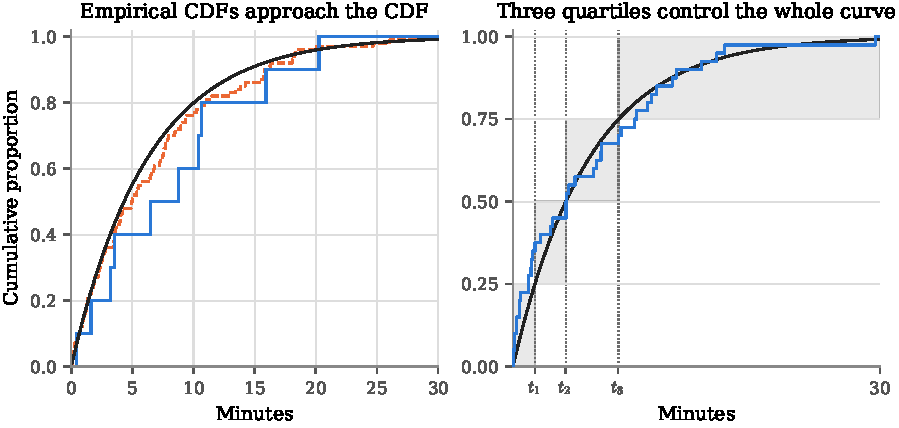
\includegraphics[width=\textwidth]{fig_ecdf_gc}
\caption{Simulated waits, mean $6.23$; the exponential CDF (black) in both halves. Left: empirical CDFs for $n = 10$ (blue) and $n = 100$ (orange, dashed). Right: quartiles $t_1, t_2, t_3$ (dotted), four gray boxes, and an empirical CDF for $n = 40$ (blue).}
\label{fig:ecdfgc}
\end{figure}

The largest gap is itself a distance between distributions, the \textbf{Kolmogorov distance} $\sup_t\abs{F(t) - G(t)}$ between the distributions with CDFs $F$ and $G$.
It compares the probabilities of the half-lines $(-\infty, t]$ only, where total variation compares those of all events, so it is never larger than the total variation distance (\cref{ex:ks-tv}).
That restriction is what makes it estimable.
\Cref{sec:dist-tv-estimate} showed that the empirical distribution of continuous data sits at total variation $1$ from the truth at every $n$; at Kolmogorov distance it converges to the truth, by the Glivenko--Cantelli theorem.
For the exponential $\Expo(1)$ and $\Gauss(1, 1)$, its closest Gaussian in KL divergence (\cref{ch:distances}), the Kolmogorov distance is $0.159$, attained at $0$, below which the Gaussian puts probability $\Phi(-1) = 0.159$ and the exponential none; their total variation distance is $0.319$.

How fast does the largest gap shrink?
In $4{,}000$ simulated samples its median is $0.247$ at $n = 10$, $0.081$ at $n = 100$ and $0.026$ at $n = 1{,}000$, and $\sqrt{n}$ times the median is close to $0.8$ at all three.
The gap shrinks like $1/\sqrt{n}$, as the error of an average does, and the next section finds the distribution of $\sqrt{n}$ times it.

\section{The size of the gap: Donsker's theorem}
\label{sec:ks-donsker}

Multiplying by $\sqrt{n}$, as the CLT does for an average, turns the gap into a random curve, $t \mapsto \sqrt{n}(F_n(t) - F(t))$.
By \cref{prop:ecdf-pointwise}, at each $t$ it is approximately $\Gauss(0, F(t)(1 - F(t)))$, and its values at two points $s \leq t$ have covariance $F(s)(1 - F(t))$.
The variance is largest where $F = \frac12$ and falls to $0$ at both ends, where $F_n$ and $F$ are both pinned near $0$ or near $1$.
For uniform data, $F(u) = u$ on $[0, 1]$, the curve is $u \mapsto \sqrt{n}(G_n(u) - u)$, with $G_n$ the empirical CDF of $n$ independent $\Unif(0, 1)$ draws $U_1, \ldots, U_n$, and the covariance at $u \leq v$ is $u(1 - v) = \min(u, v) - uv$.

\recall{The Central Limit Theorem for vectors (the vector-versions remark of \cref{ch:limit-tools}): for i.i.d.\ random vectors $Y_i$ with mean $m$ and positive definite covariance matrix $\Sigma$, $\sqrt{n}(\bar{Y}_n - m) \convd \Gauss_d(0, \Sigma)$.}

At finitely many points $u_1 < \cdots < u_k$ in $(0, 1)$, the values of this curve are $\sqrt{n}$ times the centered average of the i.i.d.\ vectors $(\ind(U_i \leq u_1), \ldots, \ind(U_i \leq u_k))$, and the CLT for vectors makes them jointly Gaussian in the limit (the covariance matrix is positive definite; \cref{ex:ks-cov} checks two points).
The limit of the whole curve is a random function with those Gaussian values.

\begin{theorem}[Kolmogorov; Donsker]
\label{thm:donsker}
Let $\Xton$ be i.i.d.\ with a continuous CDF $F$. Then
\[
\sqrt{n}\,\sup_{t \in \real}\abs{F_n(t) - F(t)} \convd K,
\]
where $K$ is the largest absolute value of a \textbf{Brownian bridge}: a random continuous function $B$ on $[0, 1]$ with $B(0) = B(1) = 0$ whose values at any points $0 < u_1 < \cdots < u_k < 1$ form a Gaussian vector with mean $0$ and $\cov(B(u), B(v)) = \min(u, v) - uv$. The distribution of $K$, \textbf{Kolmogorov's distribution}, is
\[
\Pr(K > x) = 2\sum_{j=1}^\infty (-1)^{j-1}e^{-2j^2x^2}, \qquad x > 0,
\]
and its $95\%$ quantile is $q_{0.05}(K) = 1.358$ ($1.224$ for $90\%$, $1.628$ for $99\%$).
\end{theorem}

This theorem is stated without proof.
The part about finitely many points follows from the CLT for vectors, as above; the step from finitely many points to the largest gap over all of them needs a theory of convergence for random functions that this book does not develop.
Donsker's theorem proper says that the whole curve $u \mapsto \sqrt{n}(G_n(u) - u)$ converges in distribution to $B$; this book uses only its consequence for the largest gap.
Kolmogorov (\textit{Giornale dell'Istituto Italiano degli Attuari}, 1933) found the limit distribution, and Smirnov (\textit{Annals of Mathematical Statistics}, 1948) tabulated it; Doob (\textit{Annals of Mathematical Statistics}, 1949) saw, and Donsker (\textit{Annals of Mathematical Statistics}, 1952) proved, that it is the distribution of the largest absolute value of the limiting curve, the Brownian bridge.
Notice what the limit does not depend on: $F$.
Every continuous distribution leads to the same $K$, which the next section explains.

The left of \cref{fig:brownianbridge} shows four curves $\sqrt{n}(G_n(u) - u)$ for $n = 1{,}000$ uniform draws.
They already look like the limit: pinned to $0$ at both ends, wandering most in the middle, and, like about $19$ in $20$ such curves, staying inside $\pm 1.358$.
The right compares the distribution of $\sqrt{n}$ times the largest gap at $n = 100$ with Kolmogorov's density; at $n = 100$ the exact $95\%$ point is $1.340$, against the limit's $1.358$.

\begin{figure}[htbp]
\centering
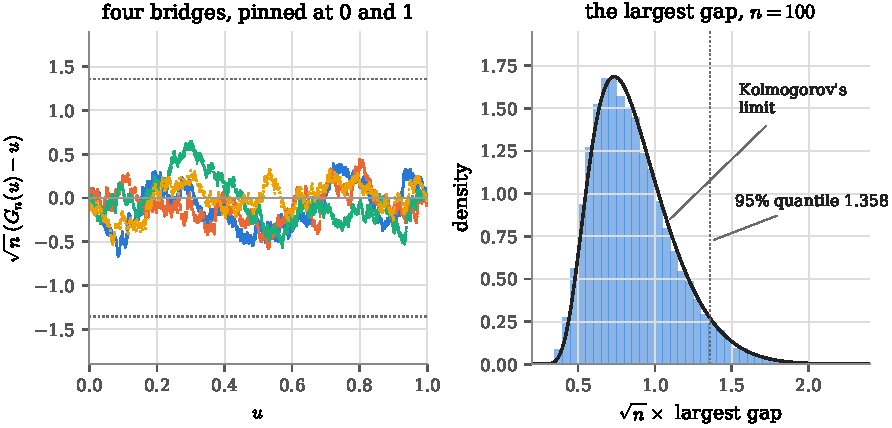
\includegraphics[width=\textwidth]{fig_brownian_bridge}
\caption{Uniform data. Left: four curves $\sqrt{n}(G_n(u) - u)$ for $n = 1{,}000$, and $\pm 1.358$ (dotted). Right: $\sqrt{n}$ times the largest gap in $20{,}000$ samples of $n = 100$ (histogram), Kolmogorov's density (black) and its $95\%$ quantile (dotted).}
\label{fig:brownianbridge}
\end{figure}

\begin{sanitycheck}[Why is the threshold 1.36 and not 0.98?]
At the single point $u = \frac12$ the bridge has variance $\frac12 - \frac14 = \frac14$, so $\abs{B(\frac12)}$ exceeds $1.96 \times \frac12 = 0.98$ with probability $5\%$.
$K$ is the largest $\abs{B(u)}$ over the whole curve, so it exceeds $0.98$ more often, and its $95\%$ point must be higher.
It is $1.358$, which is the $95\%$ point of the largest of about eight independent values distributed like $\abs{B(\frac12)}$: values of the bridge at nearby points move together, so infinitely many points behave like a handful.
The same contrast set the thresholds of the multiple-testing corrections of \cref{sec:t-multiple}: the largest of many statistics needs a larger threshold than any one of them.
\end{sanitycheck}

\textbf{A confidence band.}
For continuous $F$, since $\Pr(\sqrt{n}\sup_t\abs{F_n(t) - F(t)} \leq 1.358) \to 0.95$, the band $F_n(t) \pm 1.358/\sqrt{n}$ contains the entire curve $F$ with probability tending to $95\%$.
For Old Faithful, $n = 272$ and the half-width is $1.358/\sqrt{272} = 0.082$, so at $60$ minutes the band is $[0.223, 0.387]$, wider than the pointwise interval $[0.250, 0.360]$ of \cref{sec:ks-ecdf}, since the band must cover every $t$ at once.
The band does not even need large $n$.
Massart (\textit{Annals of Probability}, 1990) proved the Dvoretzky--Kiefer--Wolfowitz inequality with its best constant: for every $n$, every $\varepsilon > 0$ and every $F$,
\[
\Pr\Big(\sup_t\abs{F_n(t) - F(t)} > \varepsilon\Big) \leq 2e^{-2n\varepsilon^2}.
\]
Setting the right side to $0.05$ gives $\varepsilon = \sqrt{\log 40/(2n)} = 1.3581/\sqrt{n}$, the asymptotic half-width to four digits, so the band with this half-width covers $F$ with probability at least $95\%$ at every $n$, whatever $F$ is.
(The inequality is stated without proof; nothing later depends on it.)
A band tests every candidate at once: a stated CDF is rejected at the $5\%$ level when it leaves the band somewhere, and a family is rejected when every member does.
The Gaussian CDF closest to the Old Faithful staircase in Kolmogorov distance has mean $72.5$ and standard deviation $15.1$ and is $0.102$ away, outside the band, so no Gaussian fits the waits.

\section{The Kolmogorov--Smirnov test}
\label{sec:ks-test}

To test whether data come from a stated continuous distribution, measure the largest gap between its CDF and the empirical CDF.
The alternative is every other distribution, which no finite list of parameters describes; over all densities the likelihood has no maximum (a density can be made as tall as we like at the observed points), so the tests of \cref{ch:wald-lrt} do not apply, and the statistic is built from the empirical CDF alone.

\begin{definition}[The Kolmogorov--Smirnov test]
\label{def:ks-test}
Let $F^0$ be a continuous CDF. For $H_0: F = F^0$ against $H_1: F \neq F^0$, the \textbf{Kolmogorov--Smirnov statistic} is
\[
D_n = \sup_{t \in \real}\abs{F_n(t) - F^0(t)},
\]
and the \textbf{Kolmogorov--Smirnov test} of level $\alpha$ rejects when $D_n > d_\alpha(n)$, the $1 - \alpha$ quantile of $D_n$ under $H_0$. The test of asymptotic level $\alpha$ rejects when $\sqrt{n}D_n > q_\alpha(K)$, which is $1.358$ for $\alpha = 0.05$.
\end{definition}

\begin{inwords}
\textbf{In words.} Draw the candidate CDF and the staircase of the data on the same axes, find the largest vertical distance between them, and reject when it is larger than chance alone would make it. The threshold shrinks like $1/\sqrt{n}$: about $1.36/\sqrt{n}$ at the $5\%$ level.
\par\smallskip
\textbf{For the kiss data.} The kiss data are $0$s and $1$s, and the candidate $p = \frac12$ has a two-step CDF, so $D_n = \abs{F_n(0) - F^0(0)} = \abs{0.355 - 0.5} = 0.145$, the gap in the proportion of left turns, and $\sqrt{124}\,D_n = 1.62$, half the statistic $3.23$ of \cref{ch:tests-foundations}. But $F^0$ is not continuous, and the theory below does not apply: with this discrete null the threshold $1.358$ would reject a true null about $5$ times in $1{,}000$ at $n = 124$ ($0.66\%$ in the limit), not $50$ times (\cref{ex:ks-discrete}). Discrete data belong to the tests of \cref{ch:tests-foundations,ch:gof}.
\end{inwords}

The supremum runs over infinitely many $t$, but only $2n$ numbers need checking.

\begin{proposition}[Computing the statistic]
\label{prop:ks-compute}
If $F^0$ is continuous,
\[
D_n = \max_{1 \leq i \leq n}\max\Big(\frac{i}{n} - F^0(X_{(i)}),\ F^0(X_{(i)}) - \frac{i - 1}{n}\Big).
\]
\end{proposition}

\optionalproof{Between two observations the staircase is flat and $F^0$ only rises, so the largest gaps sit at the steps.}
\begin{proof}
On $[X_{(i)}, X_{(i+1)})$, $F_n = i/n$ and $F^0$ is nondecreasing, so $F_n - F^0$ is largest at the left end, where it is $i/n - F^0(X_{(i)})$, and $F^0 - F_n$ approaches its supremum $F^0(X_{(i+1)}) - i/n$ at the right end, by the continuity of $F^0$.
On $(-\infty, X_{(1)})$, $F_n = 0$ and the gap $F^0(t)$ approaches $F^0(X_{(1)}) - 0$; on $[X_{(n)}, \infty)$, $F_n = 1$ and the gap $1 - F^0(t)$ is largest at $X_{(n)}$, where it is $n/n - F^0(X_{(n)})$.
These are the $2n$ terms of the formula.
If several observations are tied, $X_{(i)} = \cdots = X_{(j)}$, the staircase jumps from $(i - 1)/n$ to $j/n$ there; the terms $j/n - F^0(X_{(j)})$ and $F^0(X_{(i)}) - (i - 1)/n$ are the gaps at that value and just below it, and the other terms of the block are no larger.
\end{proof}

\begin{worked}[ten random numbers]
A random number generator should produce independent $\Unif(0, 1)$ values.
Ten of its outputs, sorted and rounded to two decimals, are in the second row below. Here $F^0(u) = u$, so the two terms of \cref{prop:ks-compute} are the last two rows:
\begin{center}
\small
\begin{tabular}{@{}lrrrrrrrrrr@{}}
\toprule
$i$ & $1$ & $2$ & $3$ & $4$ & $5$ & $6$ & $7$ & $8$ & $9$ & $10$ \\
\midrule
$u_{(i)}$ & $0.08$ & $0.17$ & $0.38$ & $0.51$ & $0.54$ & $0.61$ & $0.80$ & $0.87$ & $0.94$ & $0.98$ \\
$i/10 - u_{(i)}$ & $0.02$ & $0.03$ & $-0.08$ & $-0.11$ & $-0.04$ & $-0.01$ & $-0.10$ & $-0.07$ & $-0.04$ & $0.02$ \\
$u_{(i)} - (i-1)/10$ & $0.08$ & $0.07$ & $0.18$ & $0.21$ & $0.14$ & $0.11$ & $0.20$ & $0.17$ & $0.14$ & $0.08$ \\
\bottomrule
\end{tabular}
\end{center}
The largest entry is $0.51 - 0.30 = 0.21$: just below $0.51$ the staircase is still at $0.30$, while the uniform CDF has reached $0.51$.
So $D_{10} = 0.21$.
The exact $5\%$ threshold for $n = 10$ is $d_{0.05}(10) = 0.409$, and the exact $p$-value is $\Pr(D_{10} \geq 0.21) = 0.70$: nothing here suggests that the generator is broken.
The asymptotic version agrees: $\sqrt{10} \times 0.21 = 0.664 < 1.358$, with $p$-value $\Pr(K > 0.664) = 0.77$.
The left of \cref{fig:ksexample} draws the staircase, the uniform CDF and this largest gap, in orange.
\end{worked}

The worked example used the uniform candidate, and nothing in it was special to the uniform.

\begin{lemma}[The probability integral transform]
\label{lem:pit}
If $X$ has a continuous CDF $F$, then $F(X) \sim \Unif(0, 1)$.
\end{lemma}

\coreproof{The event $F(X) \leq u$ is the event that $X$ is at or below the last point where $F$ equals $u$, and that has probability $u$.}
\begin{proof}
Fix $u \in (0, 1)$.
Since $F$ is continuous and runs from $0$ to $1$, it takes the value $u$ (the intermediate value theorem), and since it is nondecreasing and continuous, the set where $F(t) = u$ is a closed, bounded interval $[a, b]$, possibly a single point.
If $X \leq b$ then $F(X) \leq F(b) = u$; if $X > b$ then $F(X) > u$, since $b$ is the last point where $F$ equals $u$.
So $\Pr(F(X) \leq u) = \Pr(X \leq b) = F(b) = u$, which is the CDF of $\Unif(0, 1)$.
\end{proof}

\begin{theorem}[The Kolmogorov--Smirnov test]
\label{thm:ks}
Let $\Xton$ be i.i.d.\ with CDF $F$, and let $F^0$ be continuous.
\begin{enumerate}[nosep]
\item If $F = F^0$, then $D_n$ has the distribution of $\sup_{0 \leq u \leq 1}\abs{G_n(u) - u}$, where $G_n$ is the empirical CDF of $n$ i.i.d.\ $\Unif(0, 1)$ variables. It is the same for every continuous $F^0$, so the test of \cref{def:ks-test} has level $\alpha$, and by \cref{thm:donsker} the test with threshold $q_\alpha(K)/\sqrt{n}$ has asymptotic level $\alpha$.
\item If $F \neq F^0$, then $D_n \convp \sup_t\abs{F(t) - F^0(t)} > 0$, and the probability that either test rejects tends to $1$.
\end{enumerate}
\end{theorem}

\coreproof{Push every observation through $F^0$. Under $H_0$ the transformed values are uniform, and the vertical gaps between the staircase and the candidate do not change, since the transformation only moves points along the horizontal axis.}
\begin{proof}
(1) Suppose first that $F^0$ is strictly increasing on the interval where $0 < F^0 < 1$.
Let $U_i = F^0(X_i)$; under $H_0$ these are i.i.d.\ $\Unif(0, 1)$ by \cref{lem:pit}, and with probability $1$ every $X_i$ lies in that interval.
For such an $X_i$ and every $t$, $X_i \leq t$ exactly when $U_i \leq F^0(t)$, so $F_n(t) = G_n(F^0(t))$, where $G_n$ is the empirical CDF of $U_1, \ldots, U_n$.
Hence
\[
D_n = \sup_t\abs{G_n(F^0(t)) - F^0(t)} = \sup_{0 < u < 1}\abs{G_n(u) - u},
\]
since $F^0(t)$ takes every value in $(0, 1)$ as $t$ runs over the line; at $u = 0$ and $u = 1$ the gap is $0$ with probability $1$.
If $F^0$ is flat on a stretch, extend the stretch as far as $F^0$ stays flat: the result is a closed stretch of probability $0$.
There are at most countably many of these longest flat stretches (they do not overlap and each has positive length, so each contains a rational number of its own), so with probability $1$ no observation falls in one, endpoints included.
For every other value of $X_i$ the equivalence above still holds: if $X_i > t$ and $F^0(X_i) = F^0(t)$, then $F^0$ is flat on $[t, X_i]$, a stretch containing $X_i$.
The threshold $d_\alpha(n)$ is a quantile of this one distribution, which gives the level; and the uniform distribution is continuous, so \cref{thm:donsker} applied to $U_1, \ldots, U_n$ gives the asymptotic level.

(2) By the triangle inequality, at every $t$, $\abs{F_n(t) - F^0(t)}$ differs from $\abs{F(t) - F^0(t)}$ by at most $\abs{F_n(t) - F(t)}$, so $D_n$ differs from $c = \sup_t\abs{F(t) - F^0(t)}$ by at most $\sup_t\abs{F_n(t) - F(t)}$, which converges to $0$ in probability by \cref{thm:glivenko-cantelli}.
Hence $D_n \convp c$, and $c > 0$ since $F \neq F^0$.
Both thresholds tend to $0$: $q_\alpha(K)/\sqrt{n}$ plainly, and $d_\alpha(n)$ since, under $H_0$, the Glivenko--Cantelli theorem gives $\Pr(D_n > \varepsilon) < \alpha$ for large $n$ and any $\varepsilon > 0$, so that $d_\alpha(n) \leq \varepsilon$.
Once both thresholds are below $c/2$, the probability of rejecting is at least $\Pr(D_n > c/2)$, which tends to $1$.
\end{proof}

\begin{intuition}[one table for every continuous distribution]
The right of \cref{fig:ksexample} takes the ten generator outputs of the worked example and sends each through the exponential quantile function, $x = -5\log(1 - u)$, which turns uniform numbers into exponential waits with mean $5$ minutes (\cref{ex:ks-pit}).
Against the exponential CDF the new staircase has the same steps at the same heights, and every gap is the same, including $D_{10} = 0.21$.
That is the theorem: an increasing transformation stretches the horizontal axis and leaves heights alone, and the Kolmogorov--Smirnov statistic measures only heights.
So the null distribution of $D_n$ can be computed once, for uniform data, and used for every continuous $F^0$.
Massey (\textit{Journal of the American Statistical Association}, 1951) published such a table, for $n$ up to $35$, and a simulation of uniform samples reproduces any entry of it.
\end{intuition}

\begin{figure}[htbp]
\centering
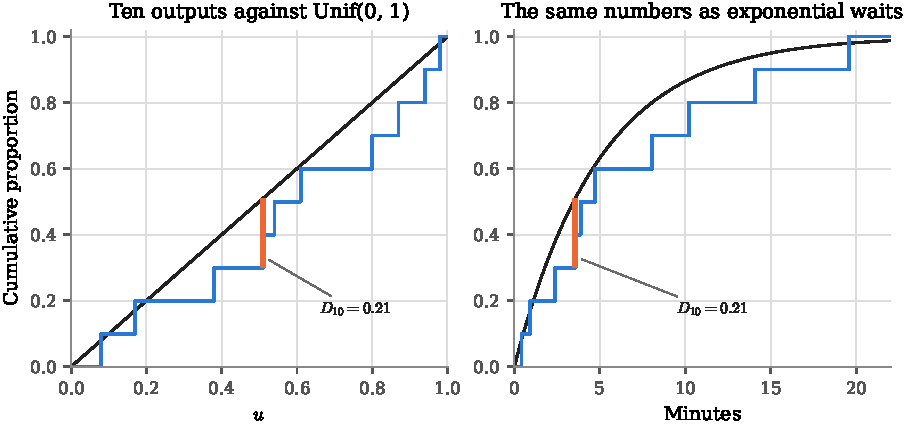
\includegraphics[width=\textwidth]{fig_ks_example}
\caption{Left: the empirical CDF (blue) of ten generator outputs against the $\Unif(0, 1)$ CDF (black), largest gap in orange. Right: the same values as exponential waits, $x = -5\log(1 - u)$, against the exponential CDF with mean $5$.}
\label{fig:ksexample}
\end{figure}

The exact thresholds approach $1.358/\sqrt{n}$ from below: for $n = 5$, $10$, $20$, $50$ and $100$ they are $0.563$, $0.409$, $0.294$, $0.188$ and $0.134$, against $0.607$, $0.429$, $0.304$, $0.192$ and $0.136$.
So the asymptotic test is slightly conservative, and from $n = 50$ on the two thresholds agree to within about $2\%$.

\section{Other measures of the gap}
\label{sec:ks-other}

The Kolmogorov--Smirnov statistic keeps only the largest gap.
Two other classical statistics add up the squared gaps over the whole line, weighting each $t$ by the probability the candidate puts near it:
\[
W^2_n = n\int_{-\infty}^\infty \big(F_n(t) - F^0(t)\big)^2 f^0(t)\,\mathrm{d}t, \qquad
A^2_n = n\int_{-\infty}^\infty \frac{\big(F_n(t) - F^0(t)\big)^2}{F^0(t)\big(1 - F^0(t)\big)}\, f^0(t)\,\mathrm{d}t,
\]
the \textbf{Cram\'er--von Mises} and \textbf{Anderson--Darling} statistics, with $f^0$ the density of $F^0$ (Anderson and Darling, \textit{Annals of Mathematical Statistics}, 1952, introduced the second).
The substitution $u = F^0(t)$, with $\mathrm{d}u = f^0(t)\,\mathrm{d}t$, turns both into integrals over $[0, 1]$ of the uniform staircase $G_n$ of \cref{thm:ks}, so both are distribution-free in the same way.
With $U_{(i)} = F^0(X_{(i)})$ they are computed as
\[
W^2_n = \frac{1}{12n} + \sum_{i=1}^n\Big(U_{(i)} - \frac{2i - 1}{2n}\Big)^2, \qquad
A^2_n = -n - \frac1n\sum_{i=1}^n(2i - 1)\Big(\log U_{(i)} + \log\big(1 - U_{(n+1-i)}\big)\Big)
\]
(\cref{ex:ks-cvm} derives the first), and their $5\%$ thresholds are about $0.46$ and $2.49$ for large $n$.

The weight in $A^2_n$ has a reason.
The gap at $t$ has variance $F(t)(1 - F(t))/n$ (\cref{prop:ecdf-pointwise}), which falls to $0$ in the tails.
The Kolmogorov--Smirnov statistic and $W^2_n$ measure raw gaps, which are naturally small in the tails, so they hardly look there.
$A^2_n$ divides each squared gap by its variance, as Pearson's statistic divided each squared deviation by its expected count in \cref{ch:gof}, and a gap in the tails then counts as much as one in the middle.

\Cref{fig:edfpower} puts the three ideas side by side for a Gaussian null with $n = 50$: the Kolmogorov--Smirnov test, the Anderson--Darling test, and Pearson's test on the counts in $4$ or in $10$ cells equally likely under the null, each with level $5\%$ or just below, its threshold simulated under the null.
When the mean is off by $0.4$ standard deviations they reject $69\%$, $78\%$, $57\%$ and $42\%$ of the time.
Binning gives something up: each observation becomes the name of its cell, and with more cells each count is noisier.
When the spread is $1.5$ times too large the order changes: $36\%$, $81\%$, $40\%$ and $60\%$.
A change of spread moves the tails most, where the Kolmogorov--Smirnov statistic hardly looks, and when the spread is $0.7$ times what it should be, the two binned tests ($47\%$ and $42\%$) beat both of the others ($17\%$ and $26\%$).
No test wins everywhere; the Anderson--Darling test loses least across these alternatives.

\begin{figure}[htbp]
\centering
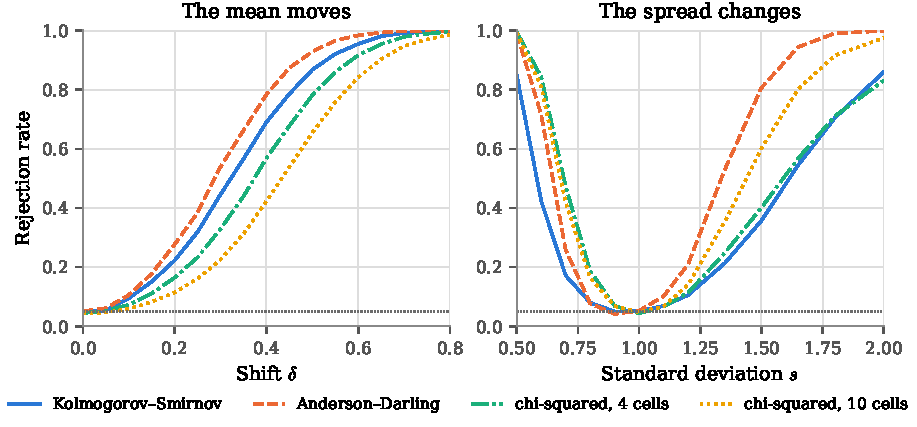
\includegraphics[width=\textwidth]{fig_edf_power}
\caption{Rejection rates of four $5\%$ tests of $\Gauss(0, 1)$ with $n = 50$: Kolmogorov--Smirnov, Anderson--Darling, and Pearson's test on $4$ or $10$ equally likely cells. Left: data from $\Gauss(\delta, 1)$. Right: data from $\Gauss(0, s^2)$. Gray dotted line: $5\%$.}
\label{fig:edfpower}
\end{figure}

\section{Testing a family: the Lilliefors test}
\label{sec:ks-lilliefors}

The question asked of data is rarely `is this $\Gauss(0, 1)$?' and usually `is this Gaussian?', with the mean and variance unknown; before the $t$-test of \cref{ch:t-test}, for instance.
The obvious move is to plug in estimates,
\[
\hat{D}_n = \sup_t\abs{F_n(t) - \Phi\Big(\frac{t - \bar{X}_n}{S_n}\Big)},
\]
with $\bar{X}_n$ and $S_n$ the sample mean and standard deviation (with divisor $n - 1$, as in \cref{ch:t-test}; the thresholds below use it), and to compare $\hat{D}_n$ with the Kolmogorov--Smirnov threshold.

\begin{pitfall}[the Kolmogorov--Smirnov table with estimated parameters]
The fitted Gaussian is chosen to match the data, so it sits closer to the empirical CDF than the true Gaussian does, and $\hat{D}_n$ is systematically smaller than $D_n$.
The left of \cref{fig:lilliefors} shows the two null distributions for $n = 50$: $95\%$ of the time $\sqrt{n}\hat{D}_n$ is below $0.88$, while the Kolmogorov--Smirnov threshold is $1.33$.
Using that threshold for $\hat{D}_n$ gives a test that rejects a true Gaussian model fewer than $2$ times in $10{,}000$ samples, at $n = 50$ and at $n = 100$ alike, where it should reject $500$ times.
\Cref{ch:gof} met the same effect for the chi-squared test: a parameter fitted to the data makes the fit look better than it is, which there cost a degree of freedom for each parameter fitted from the counts, and left no exact correction when the parameters came from the raw data (a Gaussian in four cells, compared with $\chi^2_1$ instead of $\chi^2_3$, rejected $10.5\%$ of the time in the limit instead of $5\%$: the correction overshot). For the Kolmogorov--Smirnov statistic the effect is larger, and no change of degrees of freedom repairs it.
\end{pitfall}

The repair is to find the null distribution of $\hat{D}_n$ itself, and it can be found once and for all.

\begin{proposition}[The fitted statistic is pivotal]
\label{prop:lilliefors}
Let $\Xton \iid \Gauss(\mu, \sigma^2)$, $n \geq 2$. The distribution of $\hat{D}_n$ does not depend on $\mu$ or $\sigma^2$: it is the distribution of the same statistic computed from $n$ i.i.d.\ standard Gaussians.
\end{proposition}

\coreproof{Standardize the data. Shifting and rescaling a sample shifts and rescales its empirical CDF, its mean and its standard deviation together, so every gap stays where it was.}
\begin{proof}
Write $X_i = \mu + \sigma Z_i$ with $Z_1, \ldots, Z_n \iid \Gauss(0, 1)$, and let $\bar{Z}_n$, $S^Z_n$ and $F^Z_n$ be the mean, standard deviation and empirical CDF of the $Z_i$.
Then $\bar{X}_n = \mu + \sigma\bar{Z}_n$ and $S_n = \sigma S^Z_n$.
For every $t$, put $s = (t - \mu)/\sigma$: $X_i \leq t$ exactly when $Z_i \leq s$, so $F_n(t) = F^Z_n(s)$, and $(t - \bar{X}_n)/S_n = (s - \bar{Z}_n)/S^Z_n$.
As $t$ runs over the line so does $s$, so
\[
\hat{D}_n = \sup_s\abs{F^Z_n(s) - \Phi\Big(\frac{s - \bar{Z}_n}{S^Z_n}\Big)},
\]
a function of $Z_1, \ldots, Z_n$ alone.
\end{proof}

\begin{definition}[The Lilliefors test for normality]
\label{def:lilliefors}
For $H_0$: the $X_i$ are i.i.d.\ $\Gauss(\mu, \sigma^2)$ for some $\mu$ and some $\sigma^2 > 0$, against $H_1$: they are not, the \textbf{Lilliefors test} of level $\alpha$ rejects when $\hat{D}_n > \ell_\alpha(n)$, the $1 - \alpha$ quantile of $\hat{D}_n$ under $H_0$, computed by simulating samples of $n$ standard Gaussians (\cref{prop:lilliefors}).
\end{definition}

\begin{inwords}
\textbf{In words.} Fit the Gaussian with the sample mean and standard deviation, measure the largest gap as before, and compare it with a threshold made for fitted Gaussians, about two thirds of the Kolmogorov--Smirnov one.
\par\smallskip
\textbf{For the kiss data.} The Gaussian with the kiss data's mean $0.645$ and standard deviation $0.480$ gives $\hat{D}_{124} = 0.415$, attained just below $1$, where the staircase is at $0.355$ and the fitted Gaussian at $0.770$; the $5\%$ threshold for $n = 124$ is $0.080$. Two-valued data are far from Gaussian, which is why the $t$-test of \cref{ch:t-test} is only asymptotically valid for them.
\end{inwords}

\begin{center}
\small
\begin{tabular}{@{}lrrrrr@{}}
\toprule
$n$ & $5$ & $10$ & $20$ & $50$ & $100$ \\
\midrule
Kolmogorov--Smirnov, $d_{0.05}(n)$ & $0.563$ & $0.409$ & $0.294$ & $0.188$ & $0.134$ \\
Lilliefors, $\ell_{0.05}(n)$ & $0.343$ & $0.262$ & $0.192$ & $0.125$ & $0.089$ \\
\bottomrule
\end{tabular}
\end{center}

The table gives $5\%$ thresholds for both tests; the Lilliefors values come from $200{,}000$ simulated samples for each $n$, and for large $n$ they are about $0.9/\sqrt{n}$, against $1.36/\sqrt{n}$.
Lilliefors (\textit{Journal of the American Statistical Association}, 1967) made the first such table by simulation.
The proof of \cref{prop:lilliefors} works for any family obtained by shifting and rescaling one distribution, with estimates that shift and rescale along with the data, and also for the exponential scale family (\cref{ex:ks-expo}).
For families without this invariance the null distribution depends on the true parameter, and simulating samples from the fitted distribution is the usual approximation.

\begin{worked}[Newcomb's measurements of the speed of light]
In 1882 Simon Newcomb measured, $66$ times, the time light takes to travel to a distant mirror and back, a known distance of about $7.4$ kilometers; the values are in nanoseconds above $24{,}800$ (Stigler, \textit{Annals of Statistics}, 1977).
Sixty-four of them lie between $16$ and $40$; the other two are $-44$ and $-2$.
All $66$ have mean $26.2$ and standard deviation $10.7$, and the fitted Gaussian is $\hat{D}_{66} = 0.231$ from the staircase, against the $5\%$ threshold $\ell_{0.05}(66) = 0.109$: none of $40{,}000$ simulated Gaussian samples came this far, and the test rejects.
Without the two low values, the $64$ that remain have mean $27.75$ and standard deviation $5.08$, and $\hat{D}_{64} = 0.090$ is below the threshold $\ell_{0.05}(64) = 0.111$: no evidence against a Gaussian shape.
The two values that sink the test stand out at once in the QQ plot of \cref{sec:ks-qq}.
The modern value of the speed of light corresponds to $33.0$ in these units, so the $64$ good measurements also share a systematic error of about $5$, which no test of shape can see.
\end{worked}

The right of \cref{fig:lilliefors} is the Old Faithful staircase against its fitted Gaussian, with mean $70.9$ and standard deviation $13.6$.
The fitted Gaussian puts probability $0.62$ below $75$ minutes, while only $46\%$ of the observed waits are that short; the gap, $\hat{D}_{272} = 0.155$, is almost three times the threshold $\ell_{0.05}(272) = 0.054$, and none of $20{,}000$ simulated samples came this far.
The waits are a mixture of two kinds of eruption (\cref{fig:emfaithful}), and a single Gaussian is the wrong shape.

\textbf{Rounded data.}
Newcomb's values are whole numbers and the waits are whole minutes, so both samples contain ties.
\Cref{prop:ks-compute} still computes the statistic, but rounding alone makes the staircase take bigger steps, which moves the null distribution of $\hat{D}_n$ up; the thresholds above are for unrounded data.
Gaussian samples with the fitted mean and standard deviation, rounded the same way, give $5\%$ thresholds of $0.116$ for Newcomb's $66$ values, $0.131$ for his $64$ good ones, where the $p$-value of $\hat{D}_{64} = 0.090$ rises from $0.21$ to $0.56$, and $0.063$ for the $272$ waits.
The two low values still sink Newcomb's test, the other $64$ still pass, and Old Faithful's $0.155$ is still far above its threshold.

\begin{figure}[htbp]
\centering
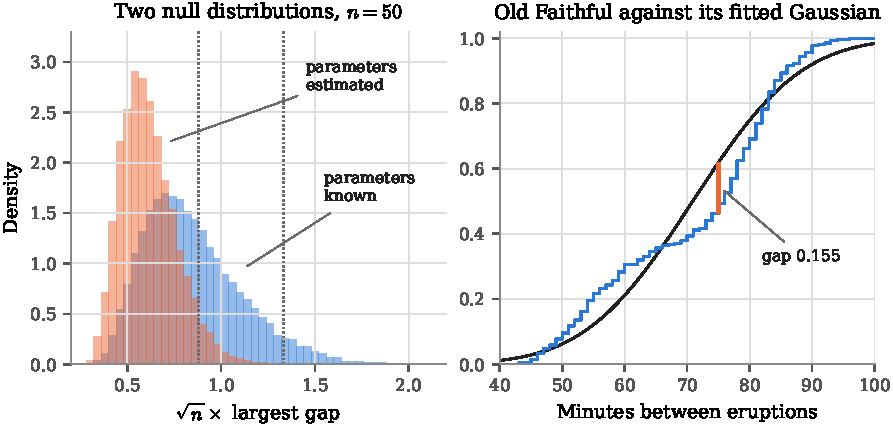
\includegraphics[width=\textwidth]{fig_lilliefors}
\caption{Left: for $n = 50$, $\sqrt{n}$ times the largest gap to the true Gaussian (blue) and the fitted one (orange); $95\%$ points $1.33$ and $0.88$ dotted. Right: Old Faithful's waits (blue), fitted Gaussian (black), largest gap (orange).}
\label{fig:lilliefors}
\end{figure}

Not rejecting is weak evidence when the sample is small.
With $12$ observations, the size of the wind-turbine sample of \cref{ch:t-test}, the Lilliefors test detects exponential data only $36\%$ of the time and data from Student's $t$ with $3$ degrees of freedom $18\%$ of the time; with $20$ observations, $58\%$ and $26\%$.

\begin{bridge}[checking normality before a $t$-test]
An introductory course asks for a look at a histogram, or a normal probability plot, before a $t$-test on a small sample, and software often reports a formal test of normality, commonly the Shapiro--Wilk test, which is more powerful than Lilliefors' against many alternatives.
The Lilliefors test is the formal version of the histogram check, and the QQ plot of the next section is the normal probability plot.
Formal tests are limited the way \cref{ch:gof} found: a small sample shows little, as the $36\%$ above says, and a large sample finds every departure, including ones that do not matter for a $t$-test, whose level the CLT protects at large $n$ (\cref{ch:t-test}).
\end{bridge}

\section{QQ plots}
\label{sec:ks-qq}

A test answers yes or no.
A QQ plot shows where the data depart from a candidate, and how.
It compares quantiles instead of CDF heights: the $i$th smallest observation $X_{(i)}$ is a sample quantile of order about $i/n$, and if the data come from $F$ it should be close to the population quantile of the same order.

\begin{definition}[QQ plot]
\label{def:qq}
Let $F$ be a continuous CDF, strictly increasing where $0 < F < 1$, with quantile function $F^{-1}$ (\cref{ch:gaussian}). The \textbf{QQ plot} of a sample against $F$ is the set of points
\[
\Big(F^{-1}\Big(\frac{i - 1/2}{n}\Big),\ X_{(i)}\Big), \qquad i = 1, \ldots, n.
\]
Against $F = \Phi$, the standard Gaussian CDF, it is called a \textbf{normal QQ plot}.
\end{definition}

\begin{inwords}
\textbf{In words.} Sort the data, and pair the $i$th smallest value with the point below which the candidate puts a fraction $(i - \frac12)/n$ of its probability. Some authors use $i/n$ and drop the last point, whose quantile $F^{-1}(1)$ is infinite; the picture is the same.
\par\smallskip
\textbf{For the kiss data.} Against Gaussian quantiles the kiss data plot as two flat rows, $44$ points at height $0$ and $80$ at height $1$. A two-valued sample gives a staircase, never a line.
\end{inwords}

If $X \sim \Gauss(\mu, \sigma^2)$, its quantile of order $p$ is $\mu + \sigma\Phi^{-1}(p)$, so the normal QQ plot of Gaussian data lies near a straight line with slope $\sigma$ and height $\mu$ at $0$, whatever $\mu$ and $\sigma$ are.
That is why one normal QQ plot checks the whole Gaussian family: the question is whether the points lie on some line, not on a particular one.
The figures below draw the line through the points at the first and third quartiles, which outliers cannot pull.

\begin{intuition}[reading the ends of a QQ plot]
For data with a single peak, the middle of a QQ plot is usually close to straight, and the ends carry the information.
\Cref{fig:qqpatterns} shows four samples of $200$ against Gaussian quantiles.
Heavy tails, as for Student's $t$ with $3$ degrees of freedom: the smallest values are smaller and the largest larger than a Gaussian with the same quartiles would give, so the left end falls below the line and the right end rises above it.
Light tails, as for the uniform: the opposite, with both ends bending back toward the horizontal.
Skewed right, as for the exponential: the lower tail is short and the upper tail long, so the points bend upward, above the line at both ends and below it in the middle.
Skewed left: the mirror image, bending down.
The skewed-right plot is the picture \cref{ch:distances} promised for exponential data and their closest Gaussian.
\end{intuition}

\begin{figure}[htbp]
\centering
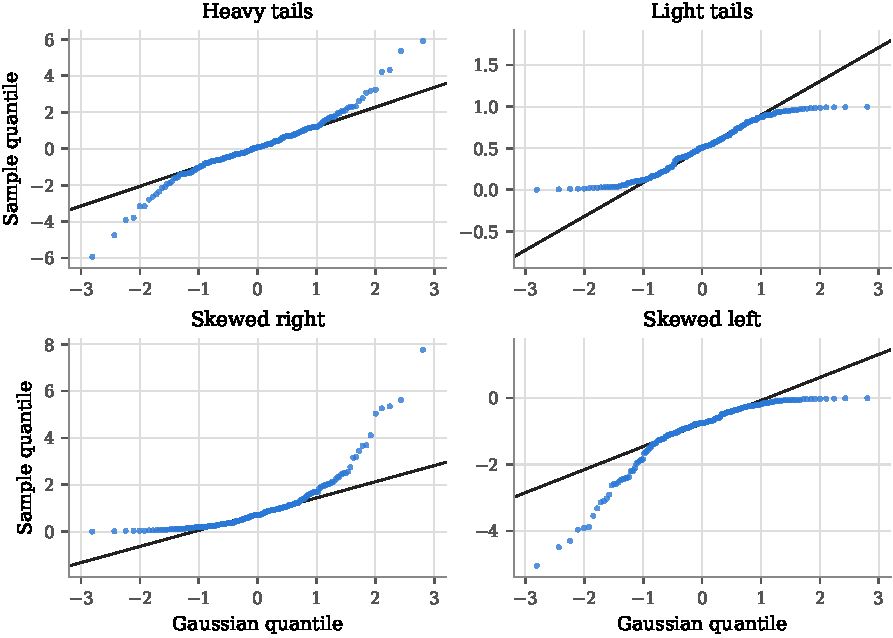
\includegraphics[width=\textwidth]{fig_qq_patterns}
\caption{Normal QQ plots of samples of $n = 200$ (blue), each with the line through its quartiles (black). Heavy tails: Student's $t$, $3$ degrees of freedom. Light tails: $\Unif(0, 1)$. Skewed right: $\Expo(1)$. Skewed left: minus an $\Expo(1)$.}
\label{fig:qqpatterns}
\end{figure}

\Cref{fig:qqreal} reads two real samples beside a simulated one.
On the left are $66$ standard Gaussians, for calibration: the points wander around the line, most at the ends, where order statistics are noisiest, and a pattern in a small sample should be judged against plots like this one.
In the middle, Newcomb's $64$ good measurements line up, and $-44$ and $-2$ sit far below the line; no test statistic points to the two culprits as directly.
On the right, Old Faithful's waits rise gently, then steeply, then gently again: two clumps, around $55$ and $80$ minutes, with few waits in between.

\begin{figure}[htbp]
\centering
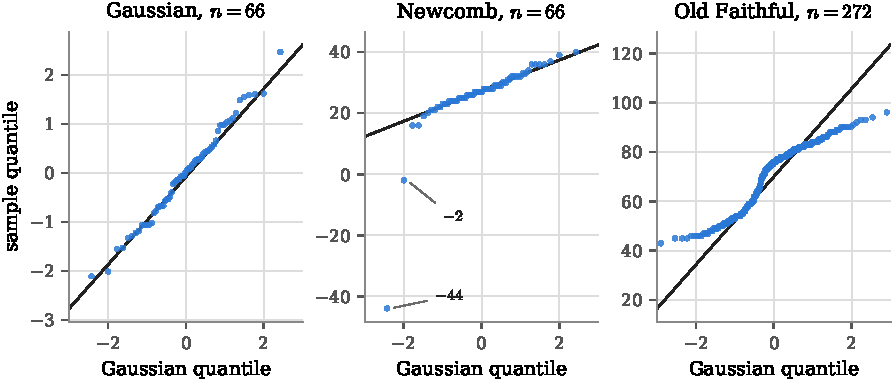
\includegraphics[width=\textwidth]{fig_qq_real}
\caption{Normal QQ plots (blue) with the line through the quartiles (black). Left: $66$ simulated standard Gaussians. Middle: Newcomb's $66$ measurements, nanoseconds above $24{,}800$. Right: Old Faithful's $272$ waits, in minutes.}
\label{fig:qqreal}
\end{figure}

The QQ plot and the Kolmogorov--Smirnov statistic compare the same two curves: the QQ plot measures the distance between them horizontally, at a fixed probability, and the statistic vertically, at a fixed $t$.
In the tails, where a CDF is nearly flat, two CDFs can be far apart horizontally and still close vertically: the extreme quantiles differ a lot while the probabilities differ little.
So the QQ plot magnifies the tails, which is where the Kolmogorov--Smirnov statistic hardly looks.

\section{What comes next}
\label{sec:ks-next}

Every method in the book so far has treated the parameter as a fixed unknown and the data as the only random thing.
\Cref{ch:bayes-intro} begins Part VII, where the parameter gets a distribution of its own: a prior, updated by the data into a posterior, with the kiss data's $p$ the first example.
The likelihood of \cref{ch:likelihood} is one of the two ingredients, and the answer is a distribution for $p$ rather than an interval or a test.

\section{Summary}
\label{sec:ks-summary}

\begin{itemize}[nosep]
\item The empirical CDF $F_n(t)$ is the proportion of the sample at or below $t$: at each $t$ a binomial proportion, with variance $F(t)(1 - F(t))/n$. Old Faithful: $F_{272}(60) = 0.305$.
\item Glivenko--Cantelli: $\sup_t\abs{F_n(t) - F(t)} \convp 0$ for every $F$, proved by cutting the line at finitely many quantiles and using monotonicity. The Kolmogorov distance can be estimated where total variation cannot.
\item Kolmogorov and Donsker: for continuous $F$, $\sqrt{n}\sup_t\abs{F_n(t) - F(t)} \convd K$, the largest absolute value of a Brownian bridge; $q_{0.05}(K) = 1.358$. The band $F_n \pm 1.358/\sqrt{n}$ covers $F$ with probability close to $95\%$ for large $n$ when $F$ is continuous, and with $1.3581$ in place of $1.358$ it covers $F$ with probability at least $95\%$ at every $n$, whatever $F$ is (Dvoretzky--Kiefer--Wolfowitz).
\item The Kolmogorov--Smirnov test of a stated continuous $F^0$ uses $D_n$, the largest of the $2n$ numbers $i/n - F^0(X_{(i)})$ and $F^0(X_{(i)}) - (i-1)/n$. By the probability integral transform its null distribution is the same for every continuous $F^0$; the test is consistent against every alternative.
\item Cram\'er--von Mises and Anderson--Darling add up squared gaps; Anderson--Darling divides each by its variance and so sees the tails. Binning for a chi-squared test loses power against shifts.
\item With parameters estimated, the Kolmogorov--Smirnov table gives a test that almost never rejects. For the Gaussian family the fitted statistic is pivotal, and the Lilliefors test simulates its null distribution: thresholds about $0.9/\sqrt{n}$ against $1.36/\sqrt{n}$. Newcomb: rejected with the two low values, not without them. Old Faithful: $0.155$ against $0.054$ ($0.063$ allowing for rounding).
\item A QQ plot pairs $X_{(i)}$ with $F^{-1}((i - \frac12)/n)$. A line means a good fit up to location and scale; heavy tails put the left end below the line and the right end above it, light tails bend both ends toward the horizontal, and skew bends the whole plot one way.
\end{itemize}

\section{Exercises}
\label{sec:ks-exercises}

\begin{exercise}
\label{ex:ks-pit}
Let $F$ be a continuous CDF, strictly increasing where $0 < F < 1$, and let $U \sim \Unif(0, 1)$. (a) Show that $F^{-1}(U)$ has CDF $F$. (b) For the exponential distribution with mean $5$, find $F^{-1}$, and turn the uniform values $0.08$ and $0.51$ into exponential waits. (c) Show that \cref{lem:pit} needs continuity: for $X \sim \Bern(\frac12)$, find the distribution of $F(X)$.
\end{exercise}
\begin{solution}
(a) For $x$ with $0 < F(x) < 1$, $F^{-1}(U) \leq x$ exactly when $U \leq F(x)$, since $F$ and $F^{-1}$ are increasing; so $\Pr(F^{-1}(U) \leq x) = \Pr(U \leq F(x)) = F(x)$. If $F(x) = 0$, then $F^{-1}(U)$, which lies where $0 < F < 1$, is above $x$, and both sides are $0$; if $F(x) = 1$, it is below $x$, and both sides are $1$. (b) $F(x) = 1 - e^{-x/5}$ for $x \geq 0$, so $F^{-1}(u) = -5\log(1 - u)$: $0.42$ and $3.57$ minutes, the first and fourth points of the right of \cref{fig:ksexample}. (c) $F(0) = \frac12$ and $F(1) = 1$, so $F(X)$ equals $\frac12$ or $1$, each with probability $\frac12$: not uniform.
\end{solution}

\begin{exercise}
\label{ex:ks-hand}
Five values are $0.8$, $0.7$, $0.4$, $0.7$ and $0.2$. Compute the Kolmogorov--Smirnov statistic for $H_0$: the data are $\Unif(0, 1)$, directly from the empirical CDF, and compare it with the exact $5\%$ threshold $d_{0.05}(5) = 0.563$ and with $1.358/\sqrt{5}$. What is odd about the data under a continuous null?
\end{exercise}
\begin{solution}
Sorted: $0.2, 0.4, 0.7, 0.7, 0.8$, so $F_5$ is $0.2$ from $0.2$, $0.4$ from $0.4$, $0.8$ from $0.7$ (two values) and $1$ from $0.8$. The gaps just below and at each step are $0.2$ and $0$ at $0.2$; $0.2$ and $0$ at $0.4$; $0.7 - 0.4 = 0.3$ and $0.8 - 0.7 = 0.1$ at $0.7$; $0$ and $0.2$ at $0.8$. So $D_5 = 0.3$, attained just below $0.7$. It is below the exact threshold $0.563$ and below $1.358/\sqrt{5} = 0.607$ (equivalently, $\sqrt{5}D_5 = 0.67 < 1.358$): do not reject. The value $0.7$ appears twice, which has probability $0$ under a continuous distribution; the data were rounded or made up. (The formula of \cref{prop:ks-compute}, applied to the five sorted values, gives the same $0.3$.)
\end{solution}

\begin{exercise}
\label{ex:ks-cov}
Let $G_n$ be the empirical CDF of $n$ i.i.d.\ $\Unif(0, 1)$ variables and $0 < u < v < 1$. (a) Show that $\sqrt{n}(G_n(u) - u)$ and $\sqrt{n}(G_n(v) - v)$ have covariance $u(1 - v)$. (b) Show that the pair converges in distribution to a Gaussian vector with this covariance, checking that the covariance matrix is positive definite. (c) Where is the limiting variance largest, and what is the correlation of the limit at $u = \frac14$ and $v = \frac34$?
\end{exercise}
\begin{solution}
(a) \Cref{prop:ecdf-pointwise} with $F(u) = u$ gives $\cov(G_n(u), G_n(v)) = u(1 - v)/n$; multiply by $n$. (b) The pair is $\sqrt{n}(\bar{Y}_n - m)$ with $Y_i = (\ind(U_i \leq u), \ind(U_i \leq v))$, $m = (u, v)$ and covariance matrix with diagonal $u(1 - u)$, $v(1 - v)$ and off-diagonal $u(1 - v)$. The diagonal is positive and the determinant is $u(1 - u)v(1 - v) - u^2(1 - v)^2 = u(1 - v)(v - u) > 0$, so the matrix is positive definite, and the CLT for vectors gives the Gaussian limit. (c) The variance $u(1 - u)$ is largest at $u = \frac12$, where it is $\frac14$. At $\frac14$ and $\frac34$ the covariance is $\frac14 \times \frac14 = \frac1{16}$ and each variance is $\frac3{16}$, so the correlation is $\frac13$.
\end{solution}

\begin{exercise}
\label{ex:ks-discrete}
For the kiss data and $F^0$ the CDF of $\Bern(\frac12)$: (a) show that $D_n = \abs{\hat{p} - \frac12}$ and that $\sqrt{n}D_n = \abs{T_n}/2$, where $T_n = \sqrt{n}(\hat{p} - \frac12)/\frac12$ is the statistic of \cref{ch:tests-foundations}; (b) under $H_0$, find the limit of $\sqrt{n}D_n$ and the limit of the probability that it exceeds $1.358$; (c) say which step of the proof of \cref{thm:ks} fails.
\end{exercise}
\begin{solution}
(a) $F_n - F^0$ is $0$ for $t < 0$ and for $t \geq 1$, and $(1 - \hat{p}) - \frac12 = \frac12 - \hat{p}$ for $0 \leq t < 1$, so $D_n = \abs{\hat{p} - \frac12}$, and $\sqrt{n}D_n = \sqrt{n}\abs{\hat{p} - \frac12} = \abs{T_n}/2$. (b) $T_n \convd \Gauss(0, 1)$ by the CLT (\cref{thm:clt}), so by the continuous mapping theorem (\cref{thm:cmt}: if $T_n \convd T$ and $g$ is continuous, $g(T_n) \convd g(T)$; here $g(t) = \abs{t}/2$), $\sqrt{n}D_n \convd \abs{Z}/2$ with $Z \sim \Gauss(0, 1)$, and $\Pr(\abs{Z}/2 > 1.358) = \Pr(\abs{Z} > 2.716) = 0.0066$. (At $n = 124$ the threshold rejects for $46$ or fewer or $78$ or more right turns, probability $0.0052$.) (c) \Cref{lem:pit}: $F^0(X)$ takes only the values $\frac12$ and $1$, so the transformed data are not uniform.
\end{solution}

\begin{exercise}
\label{ex:ks-band}
Of the $272$ Old Faithful waits, $83$ are at most $60$ minutes. (a) Compute the plug-in $95\%$ interval for $F(60)$ and the $95\%$ band of \cref{sec:ks-donsker} at $60$. (b) Why is the band wider? (c) The Gaussian CDF closest to the empirical CDF in Kolmogorov distance is $0.102$ away. What does the band say about the Gaussian family, and at what level?
\end{exercise}
\begin{solution}
(a) $0.305 \pm 1.96\sqrt{0.305 \times 0.695/272} = 0.305 \pm 0.055 = [0.250, 0.360]$, and $0.305 \pm 1.358/\sqrt{272} = 0.305 \pm 0.082 = [0.223, 0.387]$. (b) The interval covers $F(60)$ alone with probability about $95\%$; the band must cover $F(t)$ at every $t$ at once, and the largest of $\sqrt{n}\abs{F_n(t) - F(t)}$ over all $t$ is larger than its value at one point: $1.358$ against $1.96\sqrt{0.305 \times 0.695} = 0.90$ at $t = 60$. (c) Every Gaussian CDF is somewhere at least $0.102 > 0.082$ from the staircase, so every Gaussian leaves the band. If the waits were Gaussian, the band with half-width $1.3581/\sqrt{272}$, also $0.082$, would contain their CDF with probability at least $95\%$, so this rejects the whole Gaussian family at level $5\%$. (Rounding the Gaussian to the minute, as the waits are, still leaves it $0.092$ away.)
\end{solution}

\begin{exercise}
\label{ex:ks-tv}
(a) Show that the Kolmogorov distance between two distributions is at most their total variation distance. (b) For $\Expo(1)$ and $\Gauss(1, 1)$ the Kolmogorov distance is $0.159$ and the total variation distance is $0.319$; explain the value $0.159$. (c) For a sample from a continuous $F$, the empirical distribution is at total variation distance $1$ from $F$ at every $n$ (\cref{sec:dist-tv-estimate}). Why does its Kolmogorov distance from $F$ tend to $0$ all the same?
\end{exercise}
\begin{solution}
(a) Let $\Pr$ and $\Qr$ have CDFs $F$ and $G$. For each $t$, $\abs{F(t) - G(t)} = \abs{\Pr(A) - \Qr(A)}$ with $A = (-\infty, t]$, which is at most the supremum over all events, the total variation distance. (b) At $t = 0$ the Gaussian puts $\Phi(-1) = 0.159$ below $0$ and the exponential puts nothing there. For $t < 0$ the gap is $\Phi(t - 1)$, smaller still. For $t > 0$ the gap first shrinks; the exponential CDF then runs above the Gaussian one between $t = 0.26$ and $t = 2.25$, by at most $0.133$ (at $t = 0.92$, where the densities cross), and beyond $t = 2.25$ below it, by at most $0.027$ (at $t = 3.08$, where they cross again). So $0.159$ is the largest gap. (c) Total variation compares all events, including the finite set of observed values, which has empirical probability $1$ and probability $0$ under $F$. The Kolmogorov distance compares only half-lines, and \cref{thm:glivenko-cantelli} controls all of them at once.
\end{solution}

\begin{exercise}
\label{ex:ks-cvm}
Let $U_{(1)} < \cdots < U_{(n)}$ be the order statistics of $U_i = F^0(X_i)$, with $U_{(0)} = 0$ and $U_{(n+1)} = 1$. (a) Show that $W^2_n = n\int_0^1(G_n(u) - u)^2\,\mathrm{d}u$, with $G_n$ the empirical CDF of the $U_i$. (b) Using that $G_n = i/n$ on $[U_{(i)}, U_{(i+1)})$, show that $W^2_n = \frac1{12n} + \sum_i\big(U_{(i)} - \frac{2i-1}{2n}\big)^2$. (c) Compute $W^2_{10}$ for the ten generator outputs of the worked example in \cref{sec:ks-test}, and compare it with the $5\%$ threshold $0.46$.
\end{exercise}
\begin{solution}
(a) Substitute $u = F^0(t)$, $\mathrm{d}u = f^0(t)\,\mathrm{d}t$, and use $F_n(t) = G_n(F^0(t))$ from the proof of \cref{thm:ks}. (b) $\int_{U_{(i)}}^{U_{(i+1)}}(i/n - u)^2\,\mathrm{d}u = \frac13\big[(U_{(i+1)} - \frac{i}{n})^3 - (U_{(i)} - \frac{i}{n})^3\big]$. Summing over $i = 0, \ldots, n$, the terms at $U_{(0)} = 0$ and $U_{(n+1)} = 1$ vanish, and each $U_{(i)}$ with $1 \leq i \leq n$ contributes $\frac13\big[(U_{(i)} - \frac{i-1}{n})^3 - (U_{(i)} - \frac{i}{n})^3\big]$. With $a_i = U_{(i)} - \frac{2i-1}{2n}$ this is $\frac13\big[(a_i + \frac1{2n})^3 - (a_i - \frac1{2n})^3\big] = \frac{a_i^2}{n} + \frac1{12n^3}$. Multiplying the sum by $n$ gives $\sum_ia_i^2 + \frac1{12n}$. (c) The differences $a_i$ are $0.03, 0.02, 0.13, 0.16, 0.09, 0.06, 0.15, 0.12, 0.09, 0.03$, whose squares add up to $0.1014$; with $\frac1{120} = 0.0083$, $W^2_{10} = 0.110$, far below $0.46$.
\end{solution}

\begin{exercise}
\label{ex:ks-expo}
For the exponential family, let $\hat{D}_n = \sup_{t \geq 0}\abs{F_n(t) - (1 - e^{-t/\bar{X}_n})}$, the largest gap to the exponential distribution with the sample mean as its mean. Show that if the $X_i$ are i.i.d.\ $\Expo(\lambda)$, the distribution of $\hat{D}_n$ does not depend on $\lambda$, so that its thresholds can be found by simulating $\Expo(1)$ samples.
\end{exercise}
\begin{solution}
Write $X_i = Y_i/\lambda$ with $Y_1, \ldots, Y_n \iid \Expo(1)$, so $\bar{X}_n = \bar{Y}_n/\lambda$. For $t \geq 0$ put $s = \lambda t$: $X_i \leq t$ exactly when $Y_i \leq s$, so $F_n(t) = F^Y_n(s)$, and $t/\bar{X}_n = s/\bar{Y}_n$. As $t$ runs over $[0, \infty)$ so does $s$, so $\hat{D}_n = \sup_{s \geq 0}\abs{F^Y_n(s) - (1 - e^{-s/\bar{Y}_n})}$, a function of the $Y_i$ alone.
\end{solution}

\begin{exercise}
\label{ex:ks-qq-skew}
For $X \sim \Expo(1)$, the normal QQ plot of a large sample lies near the curve $h(x) = F^{-1}(\Phi(x)) = -\log(1 - \Phi(x))$. (a) Compute $h(-2)$, $h(0)$ and $h(2)$, using $\Phi(-2) = 0.023$. (b) Compare the slopes of the chords from $-2$ to $0$ and from $0$ to $2$, and explain the upward bend of the skewed-right plot in \cref{fig:qqpatterns}. (c) What is the curve for $\Unif(0, 1)$ data, and how does it explain the light-tailed plot?
\end{exercise}
\begin{solution}
(a) $h(-2) = -\log(0.977) = 0.023$, $h(0) = \log 2 = 0.693$ and $h(2) = -\log(0.023) = 3.77$. (b) The slopes are $(0.693 - 0.023)/2 = 0.335$ and $(3.77 - 0.693)/2 = 1.54$, more than four times larger on the right: the long right tail stretches the upper quantiles and the short left tail squeezes the lower ones, so the points bend upward. (c) $h(x) = \Phi(x)$, which flattens toward $0$ on the left and toward $1$ on the right: the ends of a uniform sample are closer to the middle than Gaussian ends would be, the light-tailed pattern.
\end{solution}
